% document formatting
\documentclass[10pt]{article}
\usepackage[utf8]{inputenc}
\usepackage[left=1in,right=1in,top=1in,bottom=1in]{geometry}
\usepackage[T1]{fontenc}
\usepackage{xcolor}

% math symbols, etc.
\usepackage{amsmath, amsfonts, amssymb, amsthm}

% lists
\usepackage{enumerate}

% images
\usepackage{graphicx} % for images

% code blocks
\usepackage{minted, listings} 

% verbatim greek
\usepackage{alphabeta}

\graphicspath{{./assets/images}}

\newcommand{\solution}{\textbf{Solution:}} 

\title{COM SCI M151B Week 4}

\author{Aidan Jan}
\date{\today}

\begin{document}
\maketitle

\section*{Review}
\subsection*{ISA}
\begin{itemize}
    \item First step in the design process
    \item The ISA (instruction set architecture) is essentially the assembly code.  Ex. RISC-V.
    \item ISA converts to machine code using a standard table.
\end{itemize}

\subsection*{The Iron Law of Processor Performance}
\begin{itemize}
    \item For single cycle design:
    \item $\text{CPU Time} = InstructionCount \times CyclePerInstruction \times CycleTime$
    \item Allowing for parallelism (overlaps)
    \begin{center}
        \includegraphics*[scale=0.7]{W4_1.png}
    \end{center}
\end{itemize}

\subsection*{Hazards}
\subsubsection*{Data Hazard - Read after write (RAW)}
\begin{itemize}
    \item Writing to a register (rd) and using it (rs1 or rs2) \textbf{before} the writing is finished (i.e., rd reaches to the WB stage.)
    \item To fix this, we either \textbf{stall} or \textbf{forward}.
\end{itemize}
\textbf{Stalling:}
\begin{center}
    \includegraphics*[scale=0.6]{W3_9.png}
\end{center}
\begin{itemize}
    \item We add bubble instructions (In RISC-V, this is the NOP instruction, which does nothing).
    \item Alternatively, we can add other, unrelated instructions (e.g., instructions that need to be run that don't involve any of the same registers)
\end{itemize}
\textbf{Forwarding:}
\begin{center}
    \includegraphics*[scale=0.6]{W3_11.png}
\end{center}
\begin{itemize}
    \item Instead of writing the resultant value to the register first, pass it to the ALU directly.
    \item Forwarding helps prevent stalls!
    \item See Week 3 Notes for how to detect when to forward.
\end{itemize}

\subsection*{Branches}
\begin{itemize}
    \item If we get hazards in a branch, we have two options:
    \begin{itemize}
        \item Stalling
        \item Speculation (not forwarding!)
    \end{itemize}
    \textbf{Stalling:}
    \begin{itemize}
        \item We must stall for 3 cycles!
            \begin{itemize}
                \item When: End of ID stage
                \item Where: End of EX or Beg. of Mem stage
                \item Whether: End of Mem stage
            \end{itemize}
    \end{itemize}
    \textbf{Speculation/Prediction}
    \begin{itemize}
        \item We predict which branch to take.  To do this, we predict one as always taken and the other as never taken
        \item Not taken is easier to check for, because:
        \begin{itemize}
            \item We don't need branch addresses; not taken means the next address is PC + 4.
            \item Most instructions are not branch so they are not taken too!
        \end{itemize}
        \item If we guess the branch incorrectly, we have to flush!
        \item The penalty for flushing is 3 cycles, unless we can resolve the branch during the DE stage.  This reduces the flush to 1 cycle.
    \end{itemize}
\end{itemize}

\section*{Branch Prediction}
How can we improve branch prediction?
\begin{itemize}
    \item Branch Miss Penalty
    \begin{itemize}
        \item Resolving branches sooner has reduced this penalty
    \end{itemize}
    \item Miss rate?
    \begin{itemize}
    \item Predicting always not-taken has only 30\% accuracy.
    \item What if we predict always taken?
    \begin{itemize}
        \item We need nextPC at Fetch stage!  (we need to be able to run the next instructions down that branch to save time).
    \end{itemize}
    \end{itemize}
\end{itemize}

\subsection*{Guessing Always Taken}
\begin{itemize}
    \item Idea: keep track of previous targets and use that to guess!
    \item If we see a branch instruction before, we know where it jumped.  Remember this if we see the same branch again!
    \item How frequent is this?  Is this always correct?
\end{itemize}

\subsubsection*{Branch Predictor - Where?}
\textbf{Branch Target Buffer (BTB)}
\begin{itemize}
    \item A table that stores \textit{target addresses.}
    \item Entries are indexed by PC.
    \begin{itemize}
        \item The size?  Lower bits of PC (to utilize \textit{locality}).
    \end{itemize}
\end{itemize}
\textbf{Algorithm for BTB}
\begin{itemize}
    \item For a new PC, record the target address in the table (using the PC as the index).
    \item Next time (a recurring PC), look up the table (i.e., by using the same index) and predict (i.e., use the stored value as the next PC).
\end{itemize}
\begin{center}
    \includegraphics*[scale=0.7]{W4_2.png}
\end{center}

\subsubsection*{Branch Predictor - When?}
\begin{itemize}
    \item How do we know that this is a control flow instruction?
    \begin{itemize}
        \item Since we only put control-flow instructions in the table, if the current PC matches with one entry, it is guaranteed that this instruction is a control-flow.
    \end{itemize}
    \item Who updates the BTB?
    \begin{itemize}
        \item Once the instruction is \textbf{decoded} (i.e., we realize that this is a control-flow instruction), AND the target address is known, we can update the BTB (i.e., we save both the PC and the target address.)
    \end{itemize}
\end{itemize}

\subsection*{Quick Recap}
\begin{itemize}
    \item Miss Penalty
    \begin{itemize}
        \item Move the outcome to DE
        \item Always not taken!
    \end{itemize}
    \item Miss Rate
    \begin{itemize}
        \item Always not taken is only 30\% accurate, so let's do Taken.
        \item For that we need nextPC in FE.
        \item For that we need a table (aka BTB)!
    \end{itemize}
\end{itemize}

\subsection*{Branch vs. Non-Branch}
\begin{itemize}
    \item Non-Branch (we can ignore this; next instruction is PC + 4)
    \item Branch
    \begin{itemize}
        \item Seen before (look up table)
        \item Not seen before
    \end{itemize}
\end{itemize}
\textbf{Why would this work?}\\
\begin{itemize}
    \item Two rules: \textbf{temporal} and \textbf{spatial} locality
    \begin{itemize}
        \item \textbf{Temporal Locality:} If you just did something, very likely you will do the same again \textbf{soon}!
        \item \textbf{Spatial Locality:} If you used something, very likely you will need/use similar/related things.
    \end{itemize}
    \item Programs are typically very predictable (90\% of the time spent in only 10\% of the code)
\end{itemize}
\subsection*{BTB}
\begin{center}
    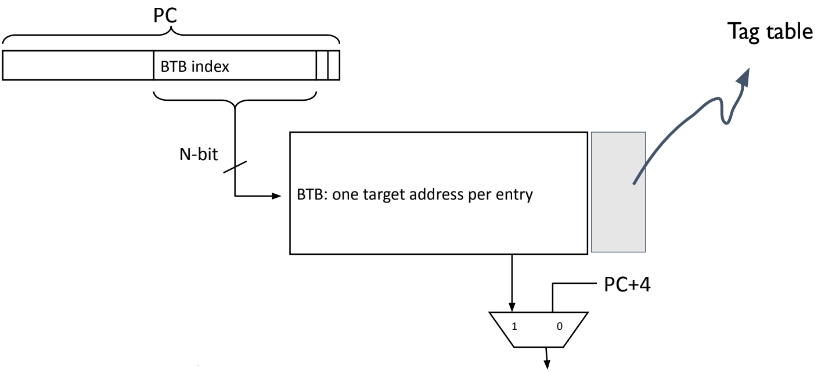
\includegraphics[scale=0.7]{W4_3.png}
\end{center}
\begin{itemize}
    \item The Tag table is implemented to make sure that the PC matches with the entry.
    \item The tag table uses the PC itself as the tag!
    \begin{itemize}
        \item (PC, target address) pairs are unique.
    \end{itemize}
\end{itemize}
\subsection*{Tagged BTB}
\begin{center}
    \includegraphics*[scale=0.7]{W4_5.png}
\end{center}
\begin{itemize}
    \item We now have a tag (PC value) that maps to the branch location.  
    \item The $N$ decides the number of entries we would have.
    \item The tag table saves a lot of memory.  With the normal BTB, if we wanted to ensure it worked for the entire code, then we would need as many entries as lines of code.  (which is a lot)
    \item Instead, we can tag only the branching statements, and store only the last $N$ bits of the instruction as a tag.  Ideally, two instructions would never have the same $N$ lower bits, but if it does, then we pay the penalty of flushing incorrect instructions.
    \item We can optimize even more!
\end{itemize}
\subsection*{Types of Control-Flow Instructions}
\begin{tabular}{|c|c|c|c|}
    \hline
    \textbf{Control Flow Inst.} & \textbf{Direction at fetch time} & \textbf{\# possible next fetch} & \textbf{When next fetch addr. resolved?}\\
    \hline
    Conditional & Unknown & 2 & Decode (rs1 == rs2)\\
    Unconditional & Always taken & 1 & Decode (PC + offset)\\
    Call & Always taken & 1 & Decode (PC + offset)\\
    Return & Always taken & Many & Decode (reg. dependent)\\
    Indirect & Always taken & Many & Decode (reg. dependent)\\
    \hline
\end{tabular}
\subsubsection*{BTB}
\begin{itemize}
    \item if r-type, i-type, lw, sw:
    \begin{itemize}
        \item PC = PC + 4 $\rightarrow$ PC won't match in BTB
    \end{itemize}
    \item if jal
    \begin{itemize}
        \item PC = PC + offset $\rightarrow$ this is what BTB would give us!
    \end{itemize}
    \item if beq
    \begin{itemize}
        \item PC = PC + offset $\rightarrow$ we still assume always-taken, but at least, we have the \textbf{address} now!
    \end{itemize}
    \item if ret, call, jalr
    \begin{itemize}
        \item PC = ? $\rightarrow$ many different possible outcomes.  BTB won't be that helpful here (it can only store one of them).
    \end{itemize}
\end{itemize}
For conditional branches we are doing always taken (70\% accurate) which is a lot better than always not taken (30\%).  \textbf{Can we do better?}

\subsection*{How to improve the prediction accuracy?}
\begin{itemize}
    \item Use a \textbf{branch predictor}
    \begin{itemize}
        \item Predict the outcome of the branch \textit{dynamically}!
    \end{itemize}
    \item How?  Use history!
    \begin{itemize}
        \item Recurring branches (e.g., backward) repeat their pattern/behavior.
        \item We can track previous branches using a table to store their outcomes; if the new branch exists in that table, use that outcome.
    \end{itemize}
\end{itemize}
\subsection*{Branch History Table (BHT)}
\begin{center}
    \includegraphics*[scale=0.8]{W4_6.png}
\end{center}
\begin{itemize}
    \item For each control statement, we store a single bit (1 or 0) on whether or not the branch was taken.
    \item For all control statements other than conditional, we store a 1, because those are always taken.
    \item For conditionals, we update the last bit \textit{based on} the last outcome of the branch.
\end{itemize}
\begin{center}
    \includegraphics*[scale=0.8]{W4_7.png}
\end{center}
\begin{itemize}
    \item Issue: they change too quickly!
    \begin{verbatim}
        Pattern:    TTTTTNTTTT
        Prediction: TTTTTTNTTT
    \end{verbatim}
    \item Even for heavily biased patterns (i.e., easy to predict), we have only 80\% accuracy.
\end{itemize}

\subsection*{Bimodal BHT (2-bit predictor)}
\begin{center}
    \includegraphics*[scale=0.8]{W4_8.png}
\end{center}
\begin{itemize}
    \item We now have better predictions!
    \begin{verbatim}
        Pattern:    TTTTTNTTTT
        Prediction: TTTTTTTTTT
    \end{verbatim}
    \item About 85-90\% accuracy for \textbf{many} programs with 2-bit counter based prediction.
    \item Need \textit{two} bits for each entry, \textbf{more overhead!}
\end{itemize}

\subsection*{Ways to Improve BHT accuracy}
\begin{itemize}
    \item Use a more complex Branch Prediction
    \item We won't get further than this, but here are some ideas:
    \begin{itemize}
        \item History of history
        \begin{itemize}
            \item Two-level prediction: all (global) and grouped (local).  Make the decision based on both patterns.
            \item Tournament: alternatively choose between global and local.
        \end{itemize}
        \item Compiler/program directed
        \begin{itemize}
            \item Use program information to train the predictor (or add some hints.)
        \end{itemize}
        \item Machine learning
        \item Hybrid
        \begin{itemize}
            \item Combine all these ideas, and dynamically pick the one that is most accurate at the time (e.g., TAGE)
        \end{itemize}
    \end{itemize}
\end{itemize}

\subsection*{Return Stack Buffer}
\begin{itemize}
    \item We have a way to deal with conditionals, unconditionals, and calls.  What about return?
    \item This is an easy problem to solve.  Keep a hardware "stack" of return addresses.
    \begin{itemize}
        \item Every time we \texttt{call} a function, push the address of the call to the stack!
        \item When return is called, we pop the last address from the stack and that will be the correct return address.
        \item This is accurate 100\% of the time!
    \end{itemize}
    \item Minor changes to BTB is needed
    \item Typically, 4-8 entries is enough, but minor changes can be made to support tail recursion.
\end{itemize}

\subsection*{What about Indirects (JALR)?}
\begin{itemize}
    \item We need additional predictors for this.
    \item However, increasing complexity adds overhead.
    \item We usually just ignore this case and tank the loss.
\end{itemize}


\end{document}
